\documentclass{standalone}

\usepackage{tikz}
\usetikzlibrary{calc,arrows}

\begin{document}
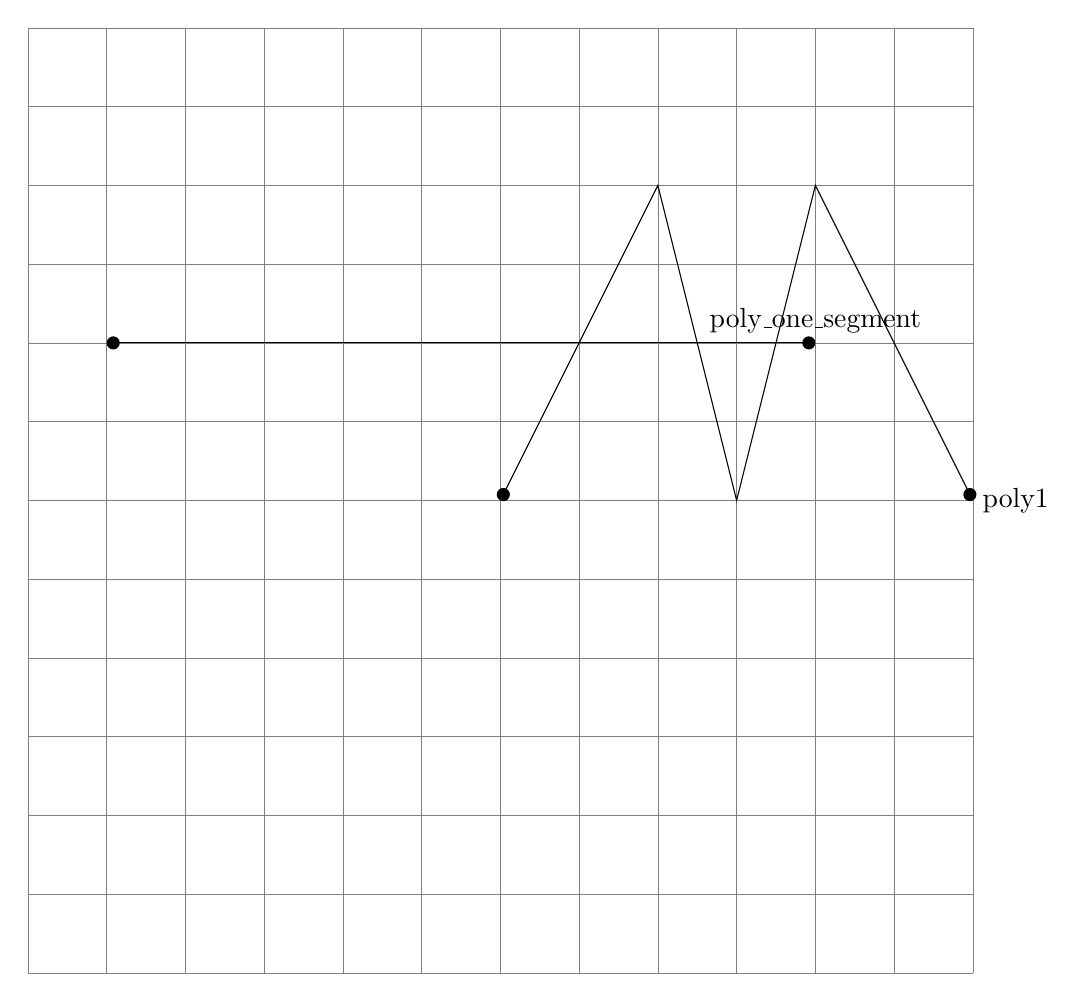
\begin{tikzpicture}
  \def\bnd{6}
  \draw[help lines] (-\bnd,-\bnd) grid (\bnd,\bnd);

  \draw[*-*] (-5,2) -- (4,2)node[above]{poly\_one\_segment};

  \draw[*-*] (0,0) -- (2,4) -- (3,0) -- (4,4) -- (6,0)node[right]{poly1};

\end{tikzpicture}
\end{document}
